%\part{Konstruktion}
%\chapter{Programmlogik}
%\section{QueryResolution}

\subsection{ResponseParse}

\begin{figure}[htb]
	\centering
		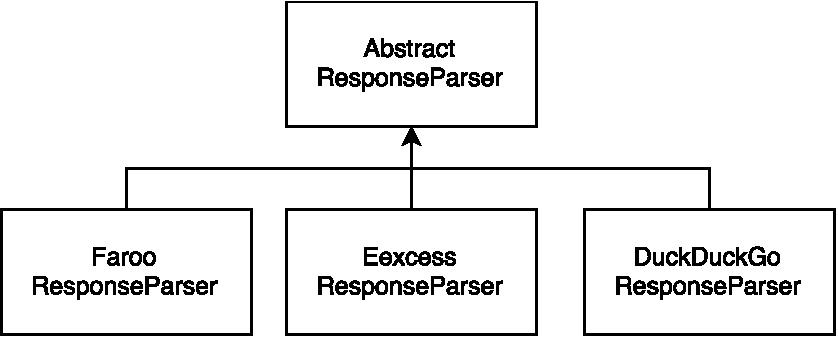
\includegraphics[width=0.8\textwidth]{response_parser}
		\caption{Aufbau des Moduls ResponseParse}
\end{figure}

Die ResponeParser sind zuständig für das Parsen der Antworten der Suchmaschinen in ein allgemeines Format.
Dabei wird in der aktuellen Version im \lstinline|AbstractResponseParser| zwischen drei spezifischen Parsern unterschieden.

\begin{itemize}
	\item \lstinline|AbstractResponseParser| spezifiziert die untergeordneten Parser
	\begin{itemize}
		\item \lstinline|FarooResponseParser| 	verarbeitet die Antworten von Faroo
		\item \lstinline|DuckDuckGoResponseParser| verarbeitet die Antworten von DuckDuckGo
		\item \lstinline|EexcessResponseParser| verarbeitet die Antworten von EEXCESS
	\end{itemize}
\end{itemize}